\documentclass[letterpaper,10pt,twoside,twocolumn,openany]{book}
\usepackage[bg=none,layout=true]{dnd}
\usepackage{dndnotes}
\usepackage{wallpaper}
\usepackage{subfiles}
\usepackage{import}
\usepackage{datetime}


\allowdisplaybreaks


\newtheorem{proposition}{Proposition}[section]
\newtheorem{axiom}{Axiom}[section]
\newenvironment{Proposition}[1]{\begin{paperbox}{}\begin{proposition}[#1]}
{\end{proposition}\end{paperbox}}
\newenvironment{Axiom}[1]{\begin{paperbox}{}\begin{proposition}[#1]}
{\end{proposition}\end{paperbox}}
\newcommand{\divides}{\ |\ }
\setcounter{secnumdepth}{1}
\graphicspath{{../Assets/}{./Assets/}}

\makeatletter
\def\input@path{{./Assets/}{../Assets/}}
\makeatother


\begin{document}
\frontmatter                           
\begin{titlepage}
    \begin{tikzpicture}[remember picture,overlay]
        \node[inner sep=0pt] at (current page.center) {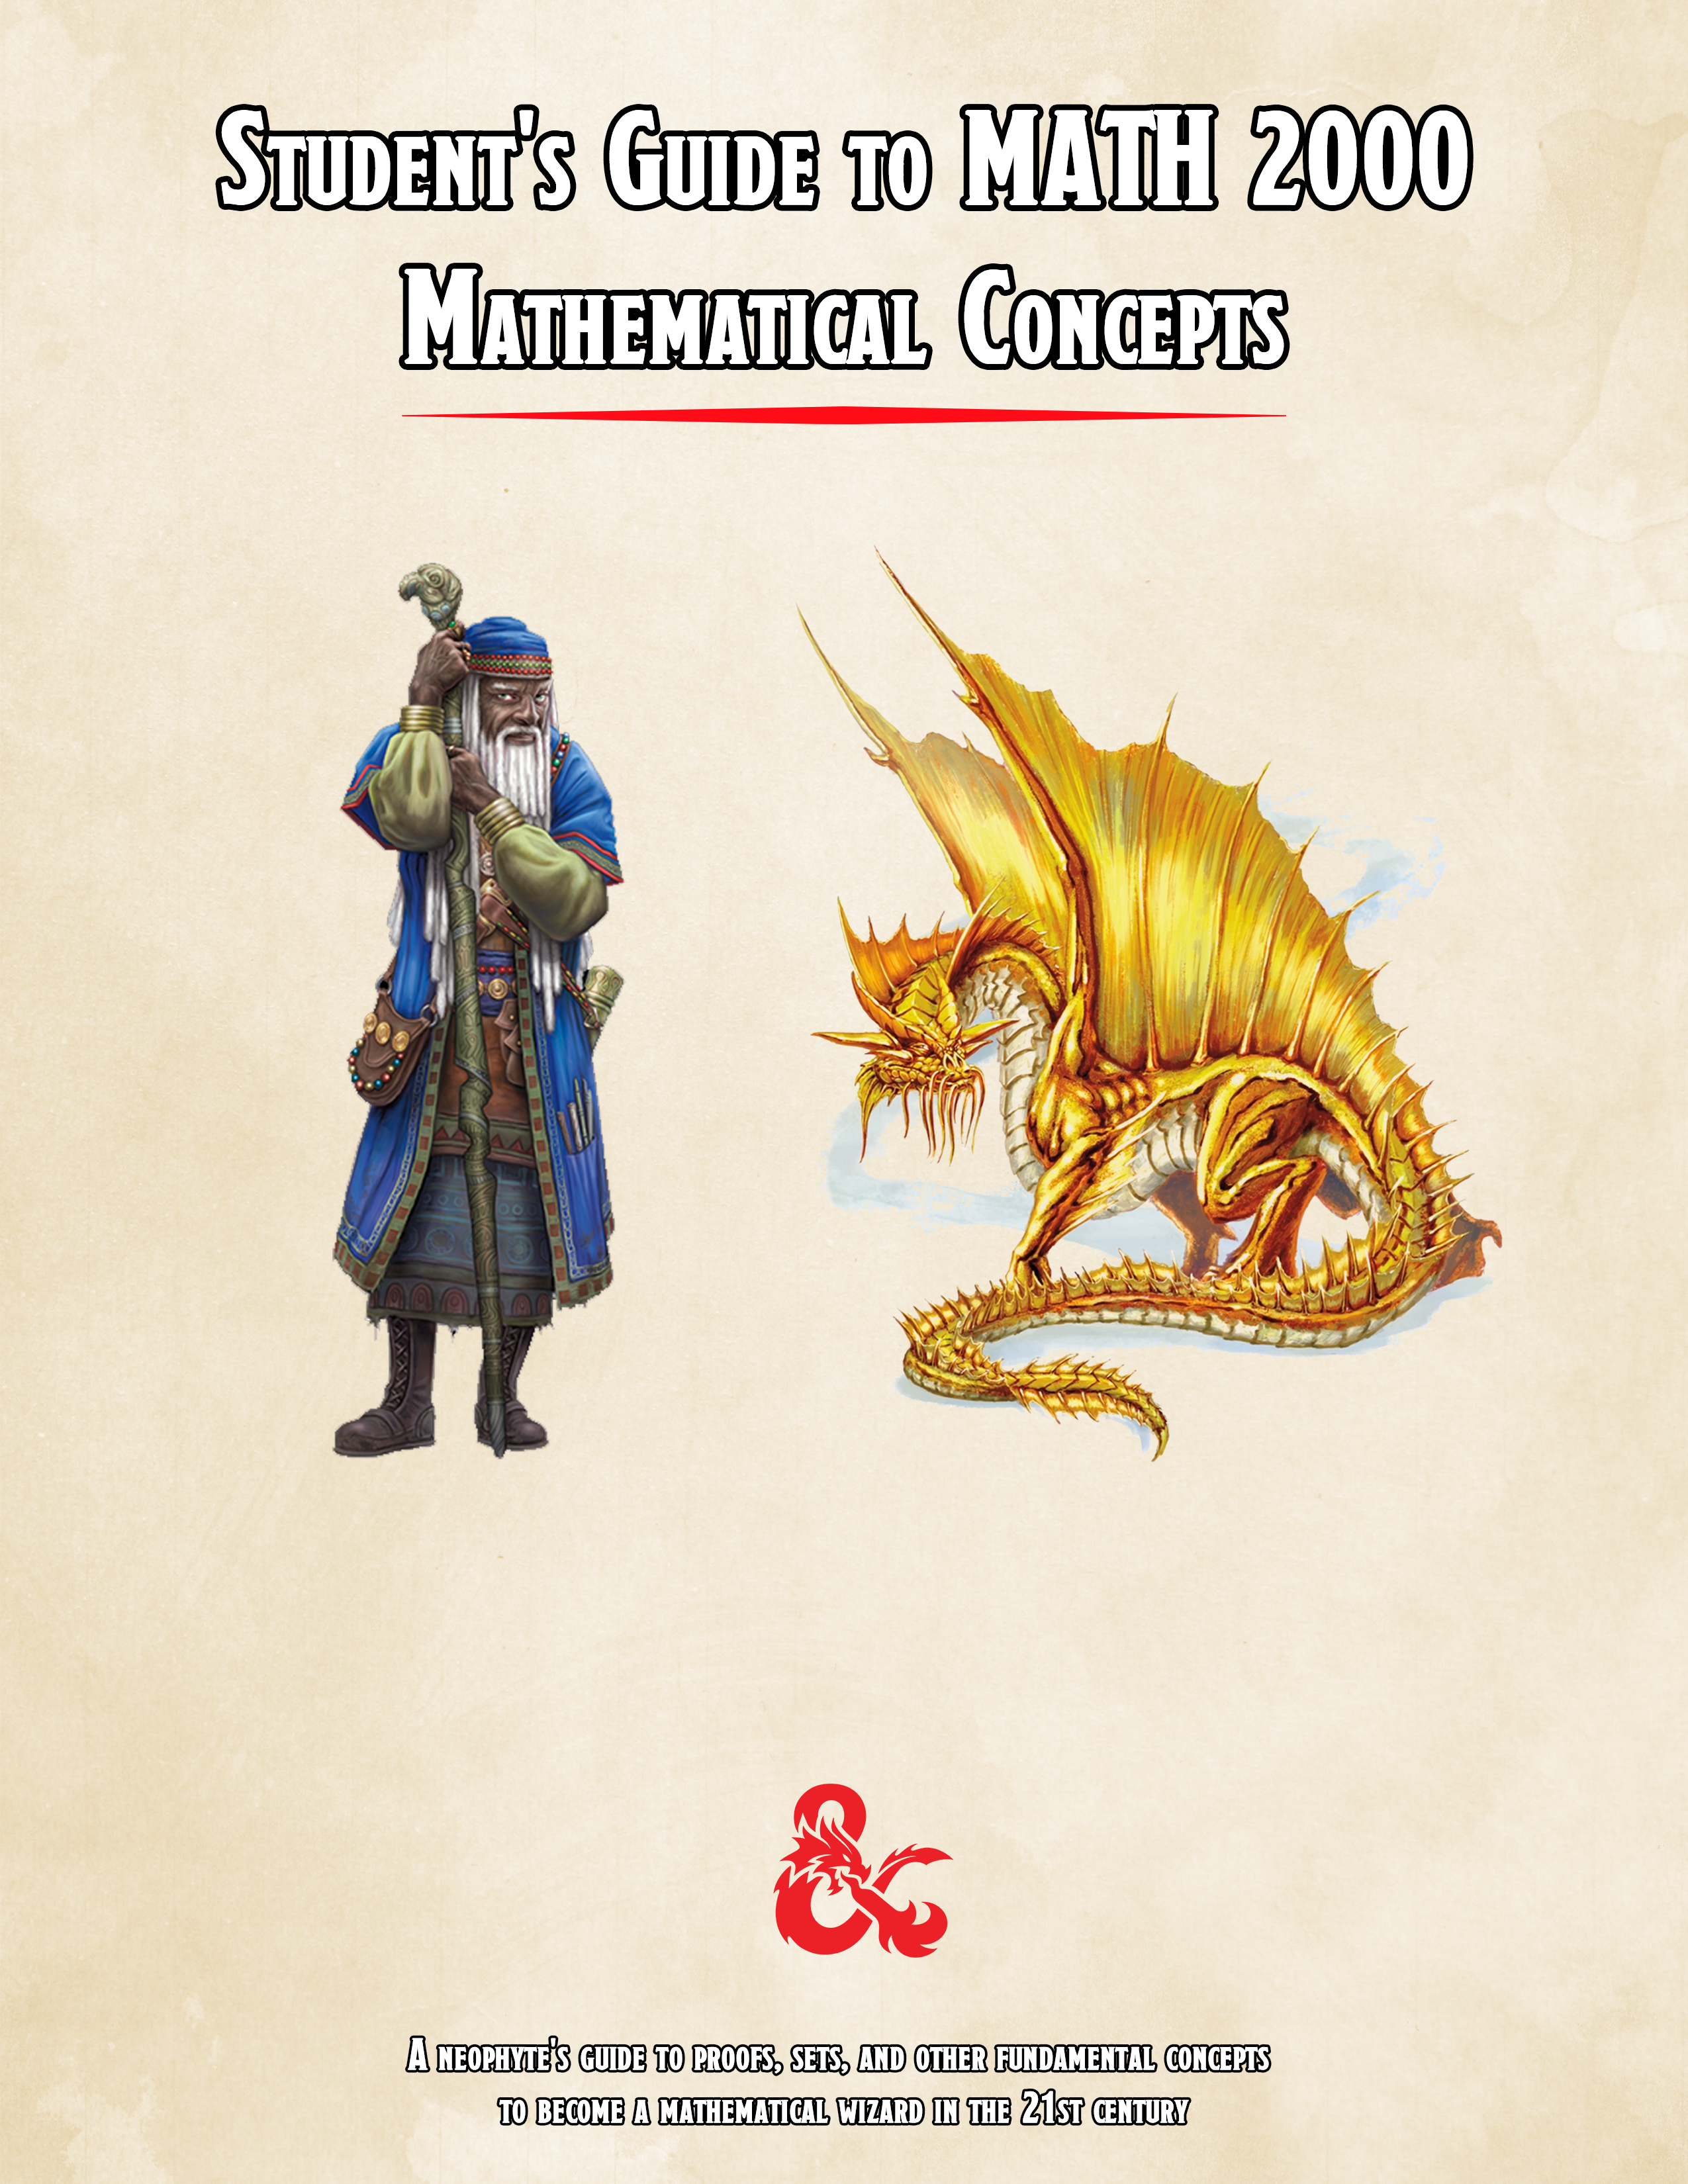
\includegraphics[width=\paperwidth,height=\paperheight]{./MATH-2000-Title.png}};
    \end{tikzpicture}~
    \newpage
    
    \begin{center}
        

        \large
        \vspace*{\fill}
        So you want to be a mathematical wizard with the dream of winning the prestigious Fields Medal or Turing award. Unlike in earlier courses where you learned the math version of cantrips, success in advanced math (and to a lesser extent CS) courses does not depend so much on being able to find the right answer to a question, but providing a convincing explanation that the answer is correct. Here you will learn what the math version of spell-casting beyond cantrips would be like. You will learn the basics of logic, proofs, set theory, relations and functions, finite and countable sets, induction, and examples of axiomatic mathematical theories.
        \vspace*{\fill}

    \end{center}
    \let\thefootnote\relax\footnote{Disclaimer: This book is not responsible for the consequences of faulty proofs, attempting to cast a mathematical fireball, speaking math cant in an examination or saying yes when the professor asks, "Are you really sure about this proof?" }
\end{titlepage}
\tableofcontents
\mainmatter
\part{Introduction to Logic and Proofs}
\subfile{Chapters/1.tex}
\subfile{Chapters/2.tex}
\part{Sets and First-Order-Logic}
\subfile{Chapters/3.tex}
\subfile{Chapters/4.tex}
\subfile{Chapters/5.tex}
\part{Other Fundamental Concepts}
\subfile{Chapters/6.tex}
\subfile{Chapters/7.tex}
\subfile{Chapters/8.tex}
\subfile{Chapters/9.tex}
\subfile{Chapters/credit.tex}
\end{document}
